\documentclass[12pt, a4paper]{ctexart}
\usepackage{geometry}
\geometry{left=2.5cm, right=2.5cm, top=3cm, bottom=3cm}
\usepackage{graphicx}
\usepackage{xcolor}
\usepackage{circuitikz}
\usepackage{subcaption}
\usepackage{float}
\usepackage{amsmath}
\usepackage{listings}
\usetikzlibrary{arrows, shapes.gates.logic.US, positioning}
\ctikzset{
    logic ports=ieee,
    logic ports/scale=0.8
}
\lstset{
    basicstyle=\ttfamily\small,
    frame=single,
    framesep=5pt,
    xleftmargin=10pt,
    xrightmargin=10pt,
    keywordstyle=\color{blue},
    commentstyle=\color{gray},
    breaklines=true
}

\begin{document}

% 封面
\begin{titlepage}
    \centering
    \vspace*{5cm}
    {\Huge\bfseries 实验报告\par}
    \vspace{2cm}
    {\Large 课程：数字逻辑与计算机组成\par}
    \vspace{1cm}
    {\Large 实验二：组合逻辑部件设计\par}
    \vspace{4cm}
    {\large 姓名：\underline{\makebox[4cm]{郑袭明}}\par}
    \vspace{1cm}
    {\large 学号：\underline{\makebox[4cm]{251502027}}\par}
    \vspace{1cm}
    {\large 日期：\today\par}
\end{titlepage}

\tableofcontents
\newpage

\section{实验目的}

\begin{enumerate}
    \item 掌握译码器、编码器、数码管等组合部件的设计方法。
    \item 掌握 1 位加法器、4 位串行加法器的设计方法。
    \item 掌握补码减法运算方法，实现补码减法功能。
    \item 掌握汉明码编码和纠错的设计方法。
    \item 掌握桶形移位器的设计方法。
\end{enumerate}

\section{实验一：译码器实验}

\subsection{整体方案设计}

该译码器的核心逻辑是将 3 位二进制输入转换为 8 个互斥的输出信号。

三个使能端必须同时有效，译码器才会工作。我们可以生成一个总使能信号

\begin{equation}
    E=G_1\cdot\overline{G_{2A,L}}\cdot\overline{G_{2B,L}}
\end{equation}

仅当 $E$ 为 1 时，译码器才会输出有效信号。

\begin{table}[H]
    \centering
    \begin{tabular}{|c|c|}
        \hline
        引脚 & 功能 \\
        \hline
        $Y_{0,L}$ & 输入位 0 低电平有效 \\
        $Y_{1,L}$ & 输入位 1 低电平有效 \\
        $Y_{2,L}$ & 输入位 2 低电平有效 \\
        $Y_{3,L}$ & 输入位 3 低电平有效 \\
        $Y_{4,L}$ & 输入位 4 低电平有效 \\
        $Y_{5,L}$ & 输入位 5 低电平有效 \\
        $Y_{6,L}$ & 输入位 6 低电平有效 \\
        $Y_{7,L}$ & 输入位 7 低电平有效 \\
        \hline
        $G_1$ & 使能端 1 \\
        $G_{2A,L}$ & 使能端 2A 低电平有效 \\
        $G_{2B,L}$ & 使能端 2B 低电平有效 \\
        \hline
        $A$ & 输入位 0 \\
        $B$ & 输入位 1 \\
        $C$ & 输入位 2 \\
        \hline
    \end{tabular}
    \caption{译码器引脚功能表}
\end{table}

\subsection{电路设计}

\begin{figure}[H]
    \centering
    \subcaptionbox{原理图}{
        \begin{circuitikz}
            \node[muxdemux,
                muxdemux def={Lh=8, Rh=8, NL=6, NB=0, NR=8},
                muxdemux label={L2=E},
                draw only left pins={2,4,5,6}
            ] (decoder) {};
            \node[and gate US, draw, logic gate inputs=nnninni, scale=1] at (-2.3,0 |- decoder.lpin 2) (and1) {};
            \draw (and1.output) -- (decoder.lpin 2);
            \node[left] (G1)at (-3.5,0 |- and1.input 1) {$G_1$};
            \node[left] (G2A) at (-3.5,0 |- and1.input 4) {$G_{2A,L}$};
            \node[left] (G2B) at (-3.5,0 |- and1.input 7) {$G_{2B,L}$};
            \draw (G1) -- (and1.input 1);
            \draw (G2A) -- (and1.input 4);
            \draw (G2B) -- (and1.input 7);
            \node[left] (A) at (decoder.lpin 4) {$A$};
            \node[left] (B) at (decoder.lpin 5) {$B$};
            \node[left] (C) at (decoder.lpin 6) {$C$};
            \node[right] (Y0) at (decoder.rpin 1) {$Y_{0,L}$};
            \node[right] (Y1) at (decoder.rpin 2) {$Y_{1,L}$};
            \node[right] (Y2) at (decoder.rpin 3) {$Y_{2,L}$};
            \node[right] (Y3) at (decoder.rpin 4) {$Y_{3,L}$};
            \node[right] (Y4) at (decoder.rpin 5) {$Y_{4,L}$};
            \node[right] (Y5) at (decoder.rpin 6) {$Y_{5,L}$};
            \node[right] (Y6) at (decoder.rpin 7) {$Y_{6,L}$};
            \node[right] (Y7) at (decoder.rpin 8) {$Y_{7,L}$};
        \end{circuitikz}
    }
    \subcaptionbox{电路图}{
\includegraphics[width=0.5\textwidth]{assets/exp1/circuit.png}}
    \caption{译码器电路设计}
\end{figure}

\subsection{仿真结果}

为了方便，我们将译码器的使能端 $E$ 的真值表和输出真值表分开列出。

\begin{table}[H]
    \centering
    \begin{tabular}{|c|ccc|cccccccc|}
        \hline
        $E$ & $A$ & $B$ & $C$ & $Y_{0,L}$ & $Y_{1,L}$ & $Y_{2,L}$ & $Y_{3,L}$ & $Y_{4,L}$ & $Y_{5,L}$ & $Y_{6,L}$ & $Y_{7,L}$ \\
        \hline
        0 & X & X & X & 1 & 1 & 1 & 1 & 1 & 1 & 1 & 1 \\ 
        \hline
        1 & 0 & 0 & 0 & 0 & 1 & 1 & 1 & 1 & 1 & 1 & 1 \\
        1 & 0 & 0 & 1 & 1 & 0 & 1 & 1 & 1 & 1 & 1 & 1 \\
        1 & 0 & 1 & 0 & 1 & 1 & 0 & 1 & 1 & 1 & 1 & 1 \\
        1 & 0 & 1 & 1 & 1 & 1 & 1 & 0 & 1 & 1 & 1 & 1 \\
        \hline
        1 & 1 & 0 & 0 & 1 & 1 & 1 & 1 & 0 & 1 & 1 & 1 \\
        1 & 1 & 0 & 1 & 1 & 1 & 1 & 1 & 1 & 0 & 1 & 1 \\
        1 & 1 & 1 & 0 & 1 & 1 & 1 & 1 & 1 & 1 & 0 & 1 \\
        1 & 1 & 1 & 1 & 1 & 1 & 1 & 1 & 1 & 1 & 1 & 0 \\
        \hline
    \end{tabular}
    \caption{译码器输出真值表}
\end{table}

\begin{table}[H]
    \centering
    \begin{tabular}{|c|c|c|c|}
        \hline
        $G_1$ & $G_{2A,L}$ & $G_{2B,L}$ & $E$ \\
        \hline
        0 & X & X & 0 \\
        X & 1 & X & 0 \\
        X & X & 1 & 0 \\
        1 & 0 & 0 & 1 \\
        \hline
    \end{tabular}
    \caption{译码器使能端 $E$ 真值表}
\end{table}

\begin{figure}[H]
    \centering
    \subcaptionbox{}{
\includegraphics[width=0.4\textwidth]{assets/exp1/sim1.png}}
    \subcaptionbox{}{
\includegraphics[width=0.4\textwidth]{assets/exp1/sim2.png}}
    \subcaptionbox{}{
\includegraphics[width=0.4\textwidth]{assets/exp1/sim3.png}}
    \subcaptionbox{}{
\includegraphics[width=0.4\textwidth]{assets/exp1/sim4.png}}
    \caption{译码器仿真结果}
\end{figure}

\subsection{错误现象及分析}

在完成实验的过程中，没有遇到任何错误。

\section{实验二：编码器实验}

\subsection{整体方案设计}

使用逻辑门实现一个 8-3 优先级编码器，可写出表达式

\begin{equation}
    \begin{aligned}
        O_0&=\overline I_0\overline I_1\overline I_2\overline I_3I_4
            +\overline I_0\overline I_1\overline I_2\overline I_3\overline I_4I_5
            +\overline I_0\overline I_1\overline I_2\overline I_3\overline I_4\overline I_5I_6
            +\overline I_0\overline I_1\overline I_2\overline I_3\overline I_4\overline I_5\overline I_6I_7
        \\ &=\overline{
            \overline{\overline I_0\overline I_1\overline I_2\overline I_3I_4}\cdot
            \overline{\overline I_0\overline I_1\overline I_2\overline I_3\overline I_4I_5}\cdot
            \overline{\overline I_0\overline I_1\overline I_2\overline I_3\overline I_4\overline I_5I_6}\cdot
            \overline{\overline I_0\overline I_1\overline I_2\overline I_3\overline I_4\overline I_5\overline I_6I_7}
        }
    \end{aligned}
\end{equation}

\begin{equation}
    \begin{aligned}
        O_1&=\overline I_0\overline I_1I_2
            +\overline I_0\overline I_1\overline I_2I_3
            +\overline I_0\overline I_1\overline I_2\overline I_3\overline I_4\overline I_5I_6
            +\overline I_0\overline I_1\overline I_2\overline I_3\overline I_4\overline I_5\overline I_6I_7
        \\ &=\overline{
            \overline{\overline I_0\overline I_1I_2}\cdot
            \overline{\overline I_0\overline I_1\overline I_2I_3}\cdot
            \overline{\overline I_0\overline I_1\overline I_2\overline I_3\overline I_4\overline I_5I_6}\cdot
            \overline{\overline I_0\overline I_1\overline I_2\overline I_3\overline I_4\overline I_5\overline I_6I_7}
        }
    \end{aligned}
\end{equation}

\begin{equation}
    \begin{aligned}
        O_2&=\overline I_0I_1
            +\overline I_0\overline I_1\overline I_2I_3
            +\overline I_0\overline I_1\overline I_2\overline I_3\overline I_4I_5
            +\overline I_0\overline I_1\overline I_2\overline I_3\overline I_4\overline I_5\overline I_6I_7
        \\ &=\overline{
            \overline{\overline I_0I_1}\cdot
            \overline{\overline I_0\overline I_1\overline I_2I_3}\cdot
            \overline{\overline I_0\overline I_1\overline I_2\overline I_3\overline I_4I_5}\cdot
            \overline{\overline I_0\overline I_1\overline I_2\overline I_3\overline I_4\overline I_5\overline I_6I_7}
        }
    \end{aligned}
\end{equation}

\begin{table}[H]
    \centering
    \begin{tabular}{|c|c|}
        \hline
        引脚 & 功能 \\
        \hline
        $I_0$ & 输入位 0 \\
        $I_1$ & 输入位 1 \\
        $I_2$ & 输入位 2 \\
        $I_3$ & 输入位 3 \\
        $I_4$ & 输入位 4 \\
        $I_5$ & 输入位 5 \\
        $I_6$ & 输入位 6 \\
        $I_7$ & 输入位 7 \\
        \hline
        $O_0$ & 输出位 0 \\
        $O_1$ & 输出位 1 \\
        $O_2$ & 输出位 2 \\
        \hline
    \end{tabular}
    \caption{编码器引脚功能表}
\end{table}

\subsection{电路设计}

\begin{figure}[H]
    \centering
    \subcaptionbox{原理图}{
        \begin{circuitikz}
            \node[muxdemux,
                muxdemux def={Lh=8, Rh=8, NL=8, NB=0, NR=3},
            ] (encoder) {};
            \node[left] (I0) at (encoder.lpin 1) {$I_0$};
            \node[left] (I1) at (encoder.lpin 2) {$I_1$};
            \node[left] (I2) at (encoder.lpin 3) {$I_2$};
            \node[left] (I3) at (encoder.lpin 4) {$I_3$};
            \node[left] (I4) at (encoder.lpin 5) {$I_4$};
            \node[left] (I5) at (encoder.lpin 6) {$I_5$};
            \node[left] (I6) at (encoder.lpin 7) {$I_6$};
            \node[left] (I7) at (encoder.lpin 8) {$I_7$};
            \node[right] (O0) at (encoder.rpin 1) {$O_0$};
            \node[right] (O1) at (encoder.rpin 2) {$O_1$};
            \node[right] (O2) at (encoder.rpin 3) {$O_2$};
        \end{circuitikz}
    }
    \subcaptionbox{电路图}{
\includegraphics[width=0.6\textwidth]{assets/exp2/circuit.png}}
    \caption{编码器电路设计}
\end{figure}

\subsection{仿真结果}

\begin{table}[H]
    \centering
    \begin{tabular}{|cccccccc|ccc|c|}
        \hline
        $I_0$ & $I_1$ & $I_2$ & $I_3$ & $I_4$ & $I_5$ & $I_6$ & $I_7$ & $O_0$ & $O_1$ & $O_2$ & Hex \\
        \hline
        1 & X & X & X & X & X & X & X & 0 & 0 & 0 & 0 \\
        0 & 1 & X & X & X & X & X & X & 0 & 0 & 1 & 1 \\
        0 & 0 & 1 & X & X & X & X & X & 0 & 1 & 0 & 2 \\
        0 & 0 & 0 & 1 & X & X & X & X & 0 & 1 & 1 & 3 \\
        \hline
        0 & 0 & 0 & 0 & 1 & X & X & X & 1 & 0 & 0 & 4 \\
        0 & 0 & 0 & 0 & 0 & 1 & X & X & 1 & 0 & 1 & 5 \\
        0 & 0 & 0 & 0 & 0 & 0 & 1 & X & 1 & 1 & 0 & 6 \\
        0 & 0 & 0 & 0 & 0 & 0 & 0 & 1 & 1 & 1 & 1 & 7 \\
        \hline
    \end{tabular}
    \caption{编码器真值表}
\end{table}

\begin{figure}[H]
    \centering
    \subcaptionbox{}{
\includegraphics[width=0.35\textwidth]{assets/exp2/sim1.png}}
    \subcaptionbox{}{
\includegraphics[width=0.35\textwidth]{assets/exp2/sim2.png}}
    \subcaptionbox{}{
\includegraphics[width=0.35\textwidth]{assets/exp2/sim3.png}}
    \subcaptionbox{}{
\includegraphics[width=0.35\textwidth]{assets/exp2/sim4.png}}
    \caption{编码器仿真结果}
\end{figure}

\subsection{错误现象及分析}

如图，在连接16进制数码显示管时，分线器多余的一位没有接上常量0，导致输出无法显示。
接上常量0后，问题得到解决。

\begin{figure}[H]
    \centering
    \subcaptionbox{改正前}{
        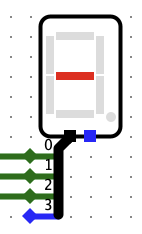
\includegraphics[width=0.15\textwidth]{assets/exp2/error1.png}
    }
    \subcaptionbox{改正后}{
        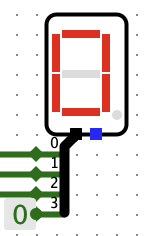
\includegraphics[width=0.15\textwidth]{assets/exp2/error2.png}
    }
    \caption{16进制数码显示管出现错误}
\end{figure}

\section{实验三：4位加法器实验}

\subsection{整体方案设计}

串联 4 个全加器子电路实现 4 位串行进位加法器，将加数、被加数和和分别连接到 16 进制数码显示管
进行验证。

\begin{figure}[H]
    \centering
    \begin{tikzpicture}[>=stealth]
        \node[draw] (fa) at (0,0) {全加器};
        \node[draw] (adder) at (3.5,0) {4 位串行加法器};
        \draw[->] (fa) -- (adder);
    \end{tikzpicture}
    \caption{4 位串行加法器设计思路}
\end{figure}

当 $Cin=1$ 时，执行补码减法运算。具体的计算原理如下

\begin{lstlisting}[language=Verilog, caption={4位加法器计算原理}]
assign {Cout, F} = A + B ^ {4{Cin}} + Cin;
\end{lstlisting}

\begin{table}[H]
    \centering
    \begin{tabular}{|c|c|}
        \hline
        引脚 & 功能 \\
        \hline
        X[3:0] & 操作数X \\
        Y[3:0] & 操作数Y \\
        Cin & 加减法切换 \\
        F[3:0] & 计算结果 \\
        Cout & 进位输出 \\
        \hline
    \end{tabular}
    \caption{4位加法器引脚功能表}
\end{table}

\subsection{电路设计}

本实验将全加器设计为一个独立的子电路，4 位串行加法器通过串联 4 个全加器实现。

\begin{figure}[H]
    \centering
    \subcaptionbox{原理图}{
        \begin{circuitikz}
            \node[muxdemux,
                muxdemux def={Lh=3, Rh=3, NL=2, NT=1, NB=1, NR=1},
            ] (adder) {};
            \node[left] (A) at (adder.lpin 1) {A};
            \node[left] (B) at (adder.lpin 2) {B};
            \node[above] (Cin) at (adder.tpin 1) {Cin};
            \node[right] (F) at (adder.rpin 1) {F};
            \node[below] (Cout) at (adder.bpin 1) {Cout};
        \end{circuitikz}
    }
    \subcaptionbox{电路图}{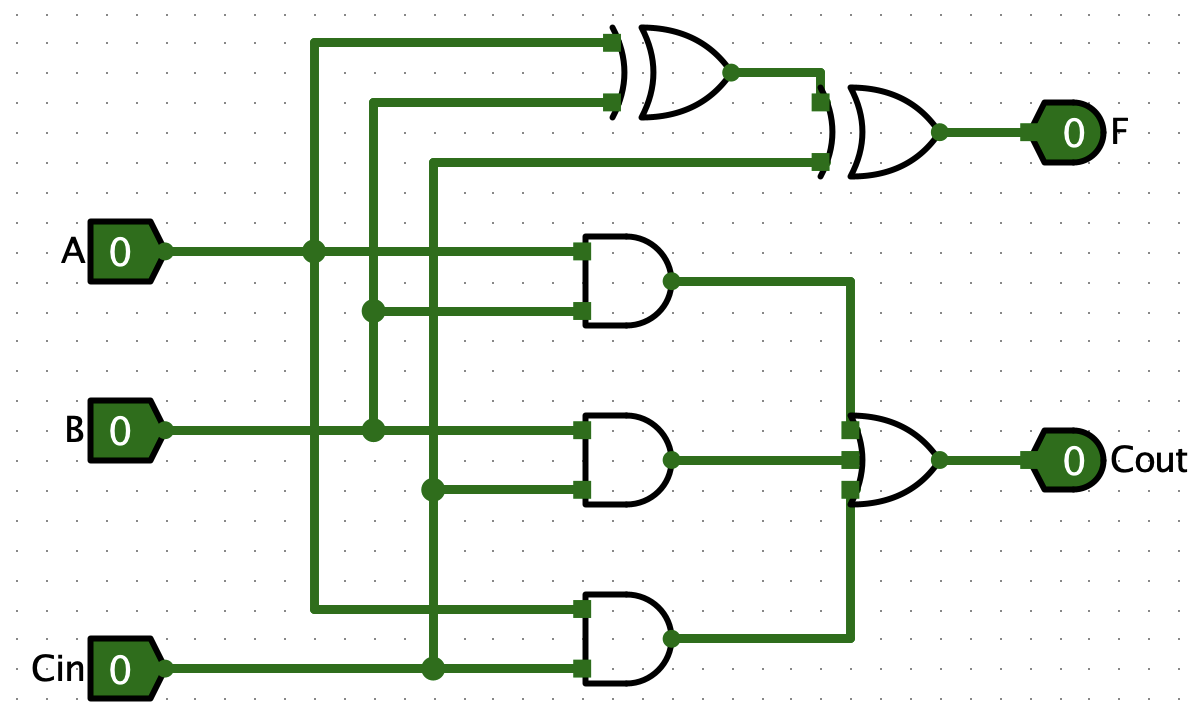
\includegraphics[width=0.4\textwidth]{assets/exp3/fa.png}}
    \caption{全加器电路设计}
\end{figure}

\begin{figure}[H]
    \centering
    \subcaptionbox{原理图}{
        \begin{circuitikz}[scale=0.8]
            \node[muxdemux,
                muxdemux def={Lh=2.5, Rh=2.5, NL=2, NT=1, NB=1, NR=1},
                muxdemux label={T1=Cin, B1=Cout}
            ] (adder1) at (0,0) {};
            \node[muxdemux,
                muxdemux def={Lh=2.5, Rh=2.5, NL=2, NT=1, NB=1, NR=1},
                muxdemux label={T1=Cin, B1=Cout}
            ] (adder2) at (0,-2) {};
            \node[muxdemux,
                muxdemux def={Lh=2.5, Rh=2.5, NL=2, NT=1, NB=1, NR=1},
                muxdemux label={T1=Cin, B1=Cout}
            ] (adder3) at (0,-4) {};
            \node[muxdemux,
                muxdemux def={Lh=2.5, Rh=2.5, NL=2, NT=1, NB=1, NR=1},
                muxdemux label={T1=Cin, B1=Cout}
            ] (adder4) at (0,-6) {};
            \node[above] (X) at (-2.2,2.2) {X};
            \node[xor gate US, draw, rotate=-90] (xor) at (-1.5,1.2) {};
            \draw (X) |- node[circ]{} (adder1.lpin 1);
            \draw (X) |- node[circ]{} (adder2.lpin 1);
            \draw (X) |- node[circ]{} (adder3.lpin 1);
            \draw (X) |- (adder4.lpin 1);
            \draw (xor.output) |- node[circ]{} (adder1.lpin 2);
            \draw (xor.output) |- node[circ]{} (adder2.lpin 2);
            \draw (xor.output) |- node[circ]{} (adder3.lpin 2);
            \draw (xor.output) |- (adder4.lpin 2);
            \node[above] (Y) at (0,2.2 -| xor.input 2) {Y};
            \node[above] (Cin) at (0,2.2) {Cin};
            \draw (Cin) -- (adder1.tpin 1);
            \draw (Cin) -- (0,1.8) node[circ]{} -| (xor.input 1);
            \draw (Y) -- (xor.input 2);
            \node[above] (F) at (1.5,2.2) {F};
            \draw (adder1.rpin 1) -| node[circ]{} (F);
            \draw (adder2.rpin 1) -| node[circ]{} (F);
            \draw (adder3.rpin 1) -| node[circ]{} (F);
            \draw (adder4.rpin 1) -| (F);
            \node[below] (Cout) at (adder4.bpin 1) {Cout};
        \end{circuitikz}
    }
    \subcaptionbox{电路图}{
\includegraphics[width=0.7\textwidth]{assets/exp3/circuit.png}}
    \caption{4位加法器电路设计}
\end{figure}

\subsection{仿真结果}

\begin{figure}[H]
    \centering
    \subcaptionbox{}{
\includegraphics[width=0.35\textwidth]{assets/exp3/sim1.png}}
    \subcaptionbox{}{
\includegraphics[width=0.35\textwidth]{assets/exp3/sim2.png}}
    \subcaptionbox{}{
\includegraphics[width=0.35\textwidth]{assets/exp3/sim3.png}}
    \subcaptionbox{}{
\includegraphics[width=0.35\textwidth]{assets/exp3/sim4.png}}
    \caption{4位加法器仿真结果}
\end{figure}

\begin{table}[H]
    \centering
    \begin{tabular}{|c|c|c|}
        \hline
        Cin & F[3:0] & Cout \\
        \hline
        0 & $X+Y$ & $X+Y\ge16$ \\
        1 & $X-Y$ & $X\ge Y$ \\
        \hline
    \end{tabular}
    \caption{4位加法器真值表}
\end{table}

\subsection{错误现象及分析}

最开始完成实验时，读题有误，认为 $Cin=1$ 时仍然执行加法运算，导致仿真结果不正确。

\section{实验四：汉明码纠错实验}

\subsection{整体方案设计}

使用奇偶校验对汉明码进行纠错，原理如下

\begin{lstlisting}[language=Verilog, caption={汉明码纠错原理}]
assign parity[0] = DU[0] ^ DU[2] ^ DU[4] ^ DU[6];
assign parity[1] = DU[1] ^ DU[2] ^ DU[5] ^ DU[6];
assign parity[2] = DU[3] ^ DU[4] ^ DU[5] ^ DU[6];
assign NOERROR = ~(parity[0] | parity[1] | parity[2]);
assign DC = NOERROR ? DU : (DU ^ (7'd1 << (parity - 3'd1)));
\end{lstlisting}

其中计算 \lstinline|parity| 的过程是通过四位异或运算进行的，可以封装成奇偶校验模块。

最后一步对 \lstinline|DC| 的计算需要使用 3-8 译码器，可以复用之前的模块设计。

\begin{figure}[H]
    \centering
    \begin{tikzpicture}[>=stealth]
        \node[draw] (parity) at (0,0) {奇偶校验模块};
        \node[draw] (hamming) at (4,0) {汉明码纠错模块};
        \node[draw] (decoder) at (4,1.5) {3-8译码器模块};
        \draw[->] (parity) -- (hamming);
        \draw[->] (decoder) -- (hamming);
    \end{tikzpicture}
    \caption{汉明码纠错设计思路}
\end{figure}

\begin{table}[H]
    \centering
    \begin{tabular}{|c|c|}
        \hline
        引脚 & 功能 \\
        \hline
        DU[6:0] & 输入数据位 \\
        NOERROR & 无错误指示 \\
        DC[6:0] & 纠错后的数据位 \\
        \hline
    \end{tabular}
    \caption{汉明码纠错引脚功能表}
\end{table}

\subsection{电路设计}

\begin{figure}[H]
    \centering
    \subcaptionbox{原理图}{
        \begin{circuitikz}[scale=0.85]
            \node[muxdemux,
                muxdemux def={Lh=2, Rh=2, NL=4, NB=0, NR=1},
                muxdemux label={L1=A,L2=B,L3=C,L4=D,R1=ODD}
            ] (parity1) at (0,0) {};
            \node[muxdemux,
                muxdemux def={Lh=2, Rh=2, NL=4, NB=0, NR=1},
                muxdemux label={L1=A,L2=B,L3=C,L4=D,R1=ODD}
            ] (parity2) at (0,-1.5) {};
            \node[muxdemux,
                muxdemux def={Lh=2, Rh=2, NL=4, NB=0, NR=1},
                muxdemux label={L1=A,L2=B,L3=C,L4=D,R1=ODD}
            ] (parity3) at (0,-3) {};
            \node[muxdemux,
                muxdemux def={Lh=2, Rh=2, NL=3, NB=0},
                muxdemux label={L1=A,L2=B,L3=C,R1=Y}
            ] (decoder) at (2.5,-1.5) {};
            \node[above] (DU) at (0,0.8 -| parity1.lpin 1) {DU[6:0]};
            \draw (DU) -- (parity3.lpin 4);
            \draw (parity1.rpin 1) -| (decoder.lpin 1);
            \draw (parity2.rpin 1) -- (decoder.lpin 2);
            \draw (parity3.rpin 1) -| (decoder.lpin 3);
            \node[xor port, anchor=in 2] (xor) at (decoder.rpin 1) {};
            \draw (DU) -| (xor.in 1);
            \node[right] (DC) at (xor.out) {DC[6:0]};
            \node[right] (NOERROR) at (4,-3) {Y[0]=NOERROR};
            \draw (decoder.rpin 1) node[circ]{} |- (NOERROR);
        \end{circuitikz}
    }
    \subcaptionbox{奇偶校验模块}{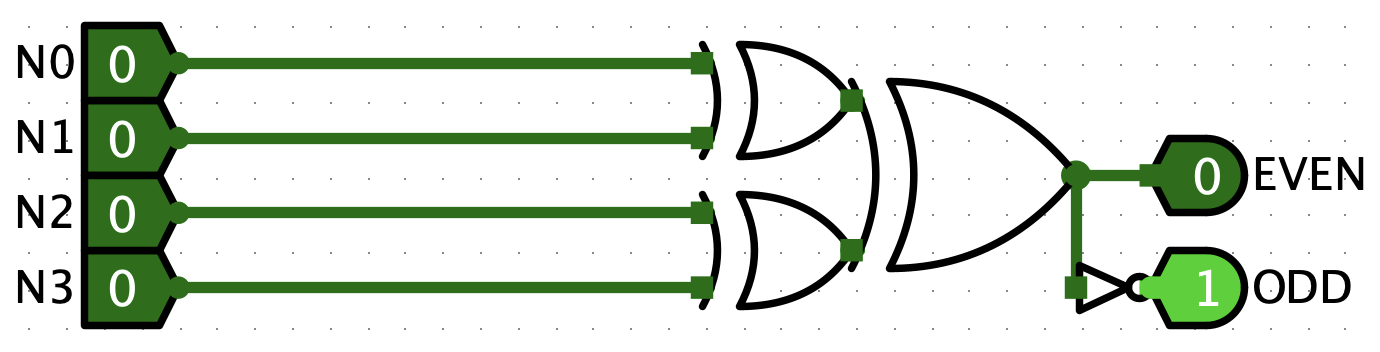
\includegraphics[width=0.4\textwidth]{assets/exp4/parity.png}}
    \subcaptionbox{电路图}{
\includegraphics[width=0.5\textwidth]{assets/exp4/circuit.png}}
    \subcaptionbox{译码器模块}{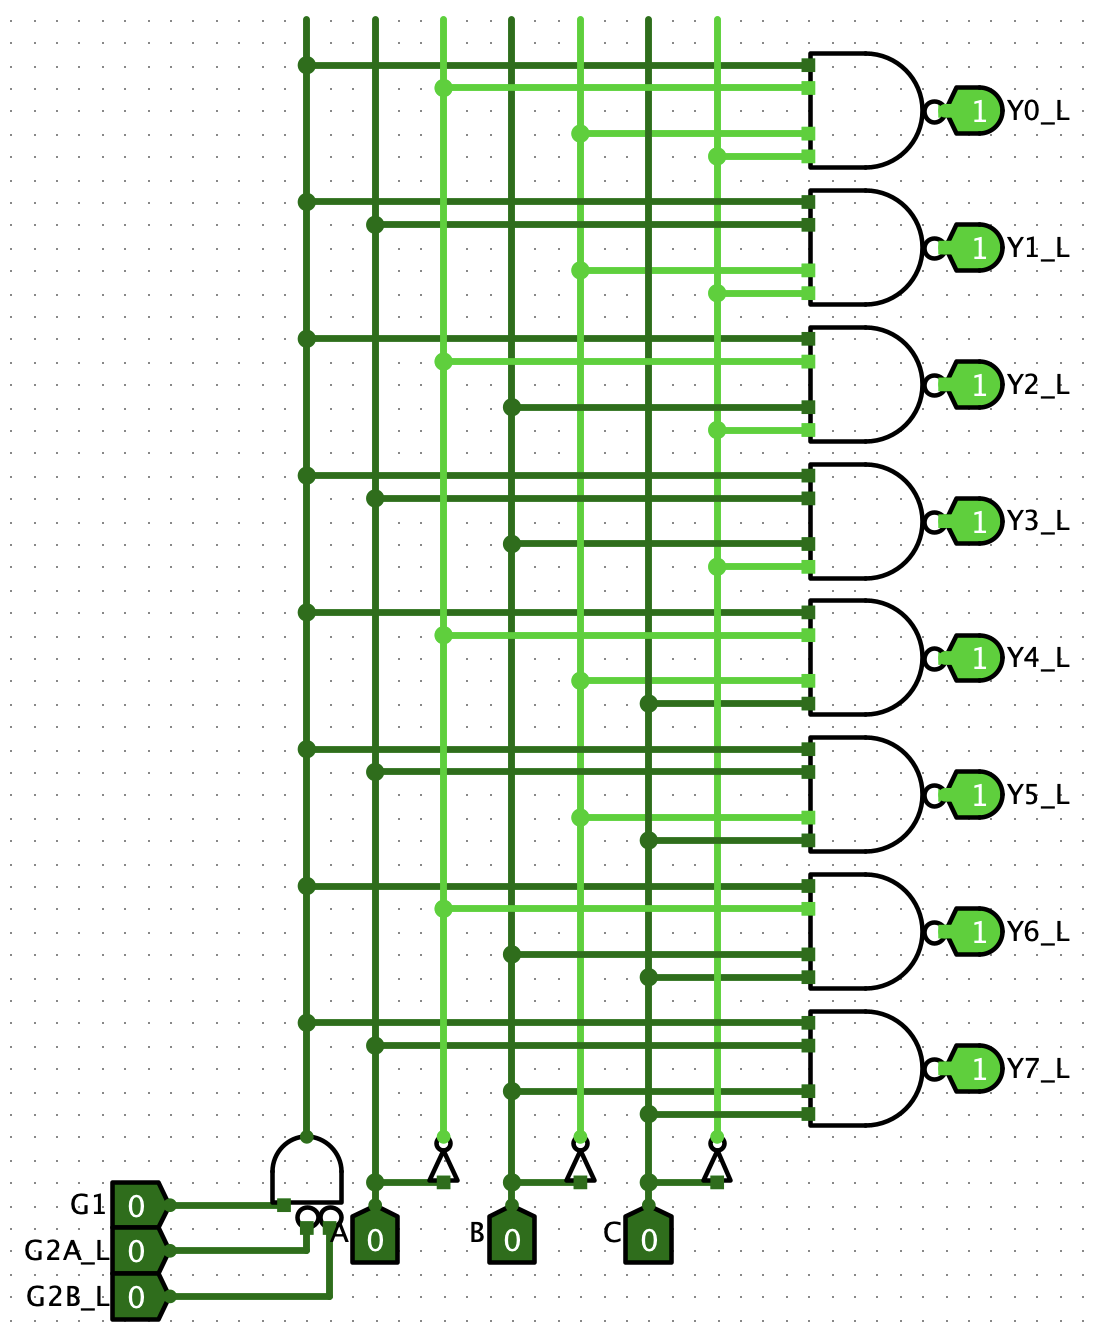
\includegraphics[width=0.35\textwidth]{assets/exp4/decoder.png}}
    \caption{汉明码纠错电路设计}
\end{figure}

\subsection{仿真结果}

\begin{figure}[H]
    \centering
    \subcaptionbox{}{
\includegraphics[width=0.4\textwidth]{assets/exp4/sim1.png}}
    \subcaptionbox{}{
\includegraphics[width=0.4\textwidth]{assets/exp4/sim2.png}}
\end{figure}

\begin{figure}[H]
    \centering
    \subcaptionbox*{(c)}{
\includegraphics[width=0.4\textwidth]{assets/exp4/sim3.png}}
    \subcaptionbox*{(d)}{
\includegraphics[width=0.4\textwidth]{assets/exp4/sim4.png}}
    \caption{汉明码纠错电路仿真结果}
\end{figure}

\subsection{错误现象及分析}

最开始没有注意到译码器的多个低电平有效的部分，导致仿真结果不正确。
后来通过检查电路发现了这个问题，加入了多个反相器后，问题得到解决。

\begin{figure}[H]
    \centering
    
\includegraphics[width=0.8\textwidth]{assets/exp4/error.png}
    \caption{汉明码纠错电路出现的错误}
\end{figure}

\section{实验五：8位桶形移位器实验}

\subsection{整体方案设计}

设计一个 8 位桶形移位器，支持算术左移、逻辑左移、算术右移和逻辑右移四种操作.（实际上只有三种）
设计原理如下

\begin{lstlisting}[language=Verilog, caption={8位桶形移位器设计原理}]
module barrel (
    input [7:0] datain,
    input [2:0] shamt,
    input lr,
    input al,
    output reg [7:0] dataout
);

  always @(*) begin
    if (lr) dataout = datain << shamt;
    else if (al) dataout = ($signed(datain)) >>> shamt;
    else dataout = datain >> shamt;
  end

endmodule
\end{lstlisting}

\begin{table}[H]
    \centering
    \begin{tabular}{|c|c|}
        \hline
        引脚 & 功能 \\
        \hline
        datain[7:0] & 输入数据位 \\
        shamt[2:0] & 移位位数 \\
        lr & 左右移选择 \\
        al & 算术/逻辑移选择 \\
        dataout[7:0] & 输出数据位 \\
        \hline
    \end{tabular}
    \caption{8位桶形移位器引脚功能表}
\end{table}

\subsection{电路设计}

\begin{figure}[H]
    \centering
    \subcaptionbox{原理图}{
        \begin{circuitikz}
            \node[muxdemux,
                muxdemux def={Lh=6, Rh=6, NL=4, NB=0, NR=1},
            ] (shifter) at (0,0) {Shifter};
            \node[left] (datain) at (shifter.lpin 1) {datain[7:0]};
            \node[left] (shamt) at (shifter.lpin 2) {shamt[2:0]};
            \node[left] (lr) at (shifter.lpin 3) {lr};
            \node[left] (al) at (shifter.lpin 4) {al};
            \node[right] (dataout) at (shifter.rpin 1) {dataout[7:0]};
        \end{circuitikz}
    }
    \subcaptionbox{电路图}{
\includegraphics[width=\textwidth]{assets/exp5/circuit.png}}
    \caption{8位桶形移位器电路设计}
\end{figure}

\subsection{仿真结果}

\begin{figure}[H]
    \centering
    \subcaptionbox{}{
\includegraphics[width=0.45\textwidth]{assets/exp5/sim1.png}}
    \subcaptionbox{}{
\includegraphics[width=0.45\textwidth]{assets/exp5/sim2.png}}
    \subcaptionbox{}{
\includegraphics[width=0.45\textwidth]{assets/exp5/sim3.png}}
    \subcaptionbox{}{
\includegraphics[width=0.45\textwidth]{assets/exp5/sim4.png}}
    \caption{8位桶形移位器仿真结果}
\end{figure}

\subsection{错误现象及分析}

由于没有仔细检查电路，导致二路选择器连反了，仿真结果不正确。
后来通过检查电路发现了这个问题，增加了反相器，问题得到解决。

\begin{figure}[H]
    \centering
    
\includegraphics[width=0.8\textwidth]{assets/exp5/error.png}
    \caption{8位桶形移位器出现的错误}
\end{figure}

\end{document}